\documentclass[11pt]{article}
\usepackage[utf8]{inputenc}
\usepackage{amsmath}
\usepackage{amsfonts}
\usepackage{amsthm}
\usepackage{amssymb}
\usepackage{mathtools}
\usepackage{physics}
\usepackage[letterpaper,margin=1.5in]{geometry}
\usepackage{cancel}
\usepackage{mathtools}
\usepackage{ulem}
\usepackage{polynom}
\usepackage{comment}
\usepackage{caption}
\usepackage{url}
\usepackage{float}
\def\ZZ{{\mathbb Z}}
\def\RR{{\mathbb R}}
\def\CC{{\mathbb C}}
\def\QQ{{\mathbb Q}}
\def\EE{{\mathbb E}}
\def\NN{{\mathbb N}}
\def\FF{{\mathbb F}}
\def\AA{{\mathcal A}}
\def\SS{{\mathbb S}}
\def\PP{{\mathbb P}}
\def\HH{{\mathbb H}}
\def\LL{{\mathcal L}}
\def\sp{{\operatorname{span}}}
\def\nul{{\operatorname{nullity}}}
\def\nu{{\operator{Null}}}
\def\ran{{\operatorname{ran}}}
\def\Int{{\operatorname{Int}}}
\def\momt{{-i\hbar \frac{d}{dx}}}
\def\hamt{{-\frac{\hbar^2}{2m} \frac{d^2}{dx^2}+V(x)}}
\DeclarePairedDelimiter\ceil{\lceil}{\rceil}
\DeclarePairedDelimiter\floor{\lfloor}{\rfloor}
\begin{document}
\begin{titlepage}
    \centering
    \vspace*{\fill}

    \vspace*{0.5cm}

    \huge\bfseries
    AMATH 271 Final Project\\
    Double Pendulum System: Coupled Oscillators and Chaos

    \vspace*{0.5cm}

    \large Yu Li \& Ryan Zhao \\
    November 2021

    \vspace*{\fill}

\end{titlepage}
\begin{abstract}
This project analyzes the double pendulum system from two distinct perspectives: coupled oscillator and chaos.
Lagrangian Mechanics is used to derive the equations of motion. Under small-angle approximations, the equations of motion
can be solved analytically, by finding the normal modes. Without approximations, the solution can only be found numerically.
Generally, the solutions are non-periodic and sensitive to initial conditions. This shows the double pendulum system exhibits chaotic behaviours.
\end{abstract}

\section{Introduction and Background}
The double pendulum system is something looks innocent and harmless: it is just a
pendulum connected to the bob of another one. But appearances are often deceptive.
Although constructed in a rather simple way, the double pendulum system exhibits
rich dynamic behaviour. In this project, we want to demonstrate the peculiar
behaviours of this system to the readers through our analysis. \\
\\
The main methodology that will be used in this project is Lagrangian Mechanics. It
is almost impossible to use Newtonian Mechanics to analyze this system by finding
out all the forces and accelerations. Lagrangian Mechanics provides us with a
simple way to derive the equations of motion, by eliminating all the forces of
constraints\cite{Taylor}.\\
\\
The first thing we are going to explore after setting up the equations of motions
is to derive the analytic solution of the system under small-angle approximations.
This is an excellent example to demonstrate the general method of analyzing
coupled oscillators, which is useful in various branches of physics\cite{Landau}.
\\
\\
Then, we will explore the behaviour of the system without approximations. The
equations of motion are impossible to solve analytically in such a
case\cite{Taylor}. The only possible way is to use computer software to find
numerical solutions. After computing the numerical solutions, we will use various
tools to analyze the solutions, such as the trajectory plots and the state-space orbits.
These are useful tools to analyze a chaotic system.
We remark that the methods used in this project
can be generalized to the analysis of other chaotic systems, so this project will
function as a demonstration of the methodologies used in the explorations of
chaos\cite{Taylor}. \\
\\
For the setup of the apparatus, please refer to Figure 1.

\pagebreak
\section{Lagrangian and Lagrange's Equations}
It is almost impossible to use Newtonian Mechanics to analyze the souble pendulum system by finding out all the forces and
accelerations. Lagrangian Mechanics is a more reasonable choice for the analysis of the system. So, we will use Lagrangian
Mechanics to analyze the double pendulum system. \\
\\
First of all, we set up the coordinate system by choosing the pivot as the origin. We choose the \(x\)-axis to be horizontally
to the right and the \(y\)-axis to be vertically upward. We use the angles between the pendulum limbs and the vertical,
\(\varphi_1\) and \(\varphi_2\), as the generalized coordinates. We assume the mass of the first pendulum bob is \(m_1\),
the mass of the second pendulum bob is \(m_2\), the length of the first pendulum limb is \(\ell_1\) and the
length of the second pendulum limb is \(\ell_2\). These setups has been illustrated in Figure 1. \\
\\
We remark that this system is holonomic, as there are two degrees of freedom (only the coordinates \(\varphi_1, \varphi_2\) can
be independently varied) and there are two generalized coordinates (\(\varphi_1\) and \(\varphi_2\)). So, the equations of motion
can be derived from Lagrange's equations.\\
\\
As we can see in Figure 1, the coordinates of the first bob is
\begin{equation*}
  x_1 = \ell_1 \sin\varphi_1
\end{equation*}
\begin{equation*}
  y_1 = -\ell_1 \cos \varphi_1
\end{equation*}
The coordinates of the second bob is
\begin{equation*}
  x_2 = \ell_1 \sin \varphi_1 + \ell_2 \sin \varphi_2
\end{equation*}
\begin{equation*}
  y_2 = -\ell_1\cos\varphi_1 - \ell_2 \cos\varphi_2
\end{equation*}
Take the total derivatives with respect to time, we have:
\begin{equation*}
  \dot{x}_1 = \ell_1 \dot{\varphi}_1 \cos\varphi_1
\end{equation*}
\begin{equation*}
  \dot{y}_1 = \ell_1 \dot{\varphi}_1 \sin \varphi_1
\end{equation*}
\begin{equation*}
  \dot{x}_2 = \ell_1 \dot{\varphi}_1 \cos\varphi_1 + \ell_2 \dot{\varphi}_2 \cos\varphi_2
\end{equation*}
\begin{equation*}
  \dot{y}_2 = \ell_1 \dot{\varphi}_1 \sin \varphi_1 + \ell_2 \dot{\varphi}_2 \sin \varphi_2
\end{equation*}
The kinetic energy of the first bob is
\begin{equation}
  T_1 = \frac{1}{2}m_1 (\dot{x}_1^2 + \dot{y}_1^2) = \frac{1}{2}m_1 \ell_1^2  \dot{\varphi}_1^2
\end{equation}
The kinetic energy of the second bob is
\begin{equation}
  T_2 = \frac{1}{2}m_2 (\dot{x}_2^2 + \dot{y}_2^2) = \frac{1}{2}m_2 (\ell_1^2  \dot{\varphi}_1^2 + \ell_2^2  \dot{\varphi}_2^2 +
  2\ell_1\ell_2\dot{\varphi}_1 \dot{\varphi}_2 \cos(\varphi_1 - \varphi_2))
\end{equation}
The gravitational potential energy of the first bob is
\begin{equation}
  U_1 = m_1gy_1 = -m_1g \ell_1 \cos \varphi_1
\end{equation}
The gravitational potential energy of the second bob is
\begin{equation}
  U_2 = m_2gy_2 = -m_2g (\ell_1\cos\varphi_1 + \ell_2 \cos\varphi_2)
\end{equation}
The Lagrangian is the total kinetic energy of the system minus the total potential energy of the system:
\begin{align*}
  \LL
  &= (T_1 + T_2) - (U_1 + U_2) \\
  &= \frac{1}{2}m_1 \ell_1^2  \dot{\varphi}_1^2 +
  \frac{1}{2}m_2 (\ell_1^2  \dot{\varphi}_1^2 + \ell_2^2  \dot{\varphi}_2^2 +
  2\ell_1\ell_2\dot{\varphi}_1 \dot{\varphi}_2 \cos(\varphi_1 - \varphi_2))\\
  &+
  m_1g \ell_1 \cos \varphi_1
  +
  m_2g (\ell_1\cos\varphi_1 + \ell_2 \cos\varphi_2)
\end{align*}
The equations of motion are derived from the Lagrange's equations. Note that there are two generalized coordinates
\(\varphi_1\) and \(\varphi_2\), so there are two equations of motion. The first equation is
\begin{equation*}
  \frac{\partial \LL}{\partial \varphi_1} = \frac{\dd}{\dd t} \frac{\partial \LL}{\partial \dot{\varphi}_1}
\end{equation*}
Substitute the expression of the Lagrangian into this equation, we have:
\begin{align*}
  &-m_2\ell_1\ell_2\dot{\varphi}_1 \dot{\varphi}_2 \sin(\varphi_1 - \varphi_2) - m_1g\ell_1 \sin\varphi_1 - m_2g\ell_1 \sin\varphi_1\\
  &= \frac{\dd}{\dd t}(m_1 \ell_1^2 \dot{\varphi}_1 + m_2 \ell_1^2 \dot{\varphi}_1 + m_2 \ell_1\ell_2 \dot{\varphi}_2\cos(\varphi_1 - \varphi_2))
\end{align*}
%\begin{align*}
%  -m_2\ell_1\ell_2\dot{\varphi}_1 \dot{\varphi}_2 \sin(\varphi_1 - \varphi_2) - (m_1+m_2)g\ell_1 \sin\varphi_1
%  &= (m_1+m_2)\ell_1^2 \ddot{\varphi}_1 + m_2 \ell_1\ell_2 \ddot{\varphi}_2\cos(\varphi_1 - \varphi_2))\\
%  &- m_2 \ell_1\ell_2 \dot{\varphi}_2\sin(\varphi_1 - \varphi_2)(\dot{\varphi}_1 - \dot{\varphi}_2)
%\end{align*}
This simplifies to
\begin{equation}
  (m_1+m_2)\ell_1 \ddot{\varphi}_1 + m_2 \ell_2 \ddot{\varphi}_2\cos(\varphi_1 - \varphi_2)
  + m_2\ell_2\dot{\varphi}_2^2 \sin(\varphi_1 - \varphi_2) + (m_1+m_2)g \sin\varphi_1 = 0
\end{equation}
The second equation is
\begin{equation*}
  \frac{\partial \LL}{\partial \varphi_2} = \frac{\dd}{\dd t} \frac{\partial \LL}{\partial \dot{\varphi}_2}
\end{equation*}
Substitute the expression of the Lagrangian into this equation, we have:
\begin{equation*}
  m_2 \ell_1\ell_2 \dot{\varphi}_1\dot{\varphi}_2\sin(\varphi_1 - \varphi_2) - m_2g\ell_2 \sin\varphi_2
  =
  \frac{\dd}{\dd t}(m_2\ell_2^2 \dot{\varphi_2} + m_2\ell_1\ell_2\dot{\varphi}_1\cos(\varphi_1-\varphi_2))
\end{equation*}
%\begin{equation*}
%  m_2\ell_1\ell_2 \dot{\varphi}_1\dot{\varphi}_2\sin(\varphi_1 - \varphi_2) - m_2g\ell_2 \sin\varphi_2
%  =
%  m_2\ell_2^2 \ddot{\varphi_2} +  m_2\ell_1\ell_2\ddot{\varphi}_1\cos(\varphi_1-\varphi_2)) -
%  m_2\ell_1\ell_2\dot{\varphi}_1\sin(\varphi_1-\varphi_2)(\dot{\varphi}_1 - \dot{\varphi}_2)
%\end{equation*}
This simplifies to
\begin{equation}
  \ell_2 \ddot{\varphi}_2 +  \ell_1\ddot{\varphi}_1\cos(\varphi_1-\varphi_2)
  -
    \ell_1\dot{\varphi}_1^2\sin(\varphi_1-\varphi_2) +  g \sin\varphi_2 = 0
\end{equation}
Overall, equation (5) and equation (6) are the equations of motion of the system.
\section{The Analytic Solution under Small-Angle Approximations}
We are going to derive the analytic solution of equation (5) and equation (6) under small-angle approximations
\(\varphi_1, \varphi_2 \ll 1\).
We will use the general method of analyzing coupled oscillators. This has been discussed in Taylor\cite{Taylor} and
Landau\cite{Landau}.
We remark that the method used here can be generalized to analyze any coupled
oscillator system, such as the oscillation of molecules\cite{Landau}. \\
\\
Under small-angle approximations, we have \(\sin(\varphi_1 -\varphi_2)\approx \varphi_1 - \varphi_2\) and
\(\cos(\varphi_1 -\varphi_2)\approx 1\). Moreover, we will neglect any products of \(\varphi_1\), \(\varphi_2\)
and their derivatives. In such a case, equation (5) and equation (6) becomes:
\begin{equation}
  (m_1+m_2)\ell_1 \ddot{\varphi}_1 + m_2 \ell_2 \ddot{\varphi}_2 + (m_1+m_2)g \varphi_1 = 0
\end{equation}
\begin{equation}
  \ell_2 \ddot{\varphi}_2 +  \ell_1\ddot{\varphi}_1+  g \varphi_2 = 0
\end{equation}
We are going to derive the analytic solution of the system of equations consisting of equation (7) and equation (8).
Note that this system of equations can be written in the following matrix form:
\begin{equation}
  M \ddot{ \varphi }(t) + K \varphi(t) = 0
\end{equation}
where
\begin{equation*}
  \varphi(t)
  =
  \begin{bmatrix}
    \varphi_1(t)\\
    \varphi_2(t)
  \end{bmatrix}
\end{equation*}
\begin{equation*}
  M =
  \begin{bmatrix}
    (m_1+m_2)\ell_1 & m_2\ell_2 \\
    \ell_1 & \ell_2
  \end{bmatrix}
\end{equation*}
\begin{equation*}
  K =
  \begin{bmatrix}
    (m_1+m_2)g & 0\\
    0 & g
  \end{bmatrix}
\end{equation*}
We see that equation (9) is the exact analog of the equation for simple harmonic oscillators \(m\ddot{x}+kx =0\), where
\(M\) corresponds to the mass \(m\) and \(K\) corresponds to the spring constant \(k\).
According to Chapter 11 of Taylor\cite{Taylor}, we should look for solutions of the form \(\varphi(t) = (a_1, a_2)^T e^{i\omega t}\),
where \(a_1, a_2\in \CC\), and then take the real part. This is called a normal mode. The general solution of the system will be the linear combination of all the normal modes.\\
\\
Substitute \(\varphi(t) = (a_1, a_2)^T e^{i\omega t}\) into equation (9), we have:
\begin{equation*}
  -\omega^2 M \varphi(t) + K\varphi(t) = 0
\end{equation*}
\begin{equation}
  (-\omega^2 M + K)\varphi(t) = 0
\end{equation}
We are looking for untrivial solutions. According to the theory of systems of linear equations, equation (10) has a non-zero solution
when
\begin{equation}
  \det(-\omega^2 M + K) = 0
\end{equation}
which is
\begin{equation*}
  \begin{vmatrix}
    -\omega^2 (m_1+m_2)\ell_1 + (m_1+m_2)g & -\omega^2 m_2\ell_2 \\
    -\omega^2 \ell_1 & -\omega^2 \ell_2 + g
  \end{vmatrix}
  = 0
\end{equation*}
Expand this determinant, we have:
\begin{equation*}
  \omega^4 m_1 \ell_1\ell_2 -  \omega^2 (m_1+m_2)(\ell_1+\ell_2)g  +(m_1+m_2)g^2  =0
\end{equation*}
This is a quadratic equation about \(\omega^2\). The solutions are:
\begin{equation}
  \omega^2_{1,2} = \frac{g }{2 \ell_1\ell_2 } \left((1+\frac{m_2}{m_1})(\ell_1+\ell_2) \pm \sqrt{(1+\frac{m_2}{m_1})((1+\frac{m_2}{m_1})(\ell_1+\ell_2)^2 - 4\ell_1\ell_2)}\right)
\end{equation}
These are the frequencies for the normal modes. Consider the case \(\ell_1\ge \ell_2\). When \(m_1\gg m_2\), we have:
\begin{equation*}
  \omega_1^2 \approx \frac{g}{2\ell_1\ell_2}((\ell_1+\ell_2) + \sqrt{(\ell_1^2+\ell_2^2 - 2\ell_1\ell_2 )}) = \frac{g}{\ell_2}
  \implies \omega_1 \approx \sqrt{\frac{g}{\ell_2}}
\end{equation*}
\begin{equation*}
  \omega_2^2 \approx \frac{g}{2\ell_1\ell_2}((\ell_1+\ell_2) - \sqrt{(\ell_1^2+\ell_2^2 - 2\ell_1\ell_2 )}) = \frac{g}{\ell_1}
  \implies \omega_2 \approx \sqrt{\frac{g}{\ell_1}}
\end{equation*}
(We directly take the square roots because frequencies are assumed to be positive.)
A similar computation shows that when \(\ell_2 >\ell_1\) and \(m_1\gg m_2\), we have \(\omega_1 \approx \sqrt{\frac{g}{\ell_1}}\)
and \(\omega_2 \approx \sqrt{\frac{g}{\ell_2}}\). We see that these are the frequencies of the simple pendulums with
length \(\ell_1\) and \(\ell_2\) under small angle approximations.
So, in such a case, the two pendulum bobs oscillate independently like simple pendulums.
This is consistent with the intuition that when \(m_1\) is so heavy, it will be virtually identical to a fixed pivot,
and the two pendulum bobs will oscillate independently like simple pendulums.\\
\\
Theoretically, we can substitute the expressions of \(\omega^2\) given by equation (12) into equation (10) to find out the corresponding \((a_1, a_2)^T\) vectors.
Then, the general solution will be all possible linear combinations of the normal modes \(\Re((a_1, a_2)^T e^{i\omega t})\).
But in reality, the computation is too cumbersome to carry out. So, to demonstrate the procedure
of finding the \((a_1, a_2)^T\) vectors, we will assume \(\ell_1=\ell_2 =\ell\) and \(m_1=m_2=m\) in our expressions.
This corresponds to a double pendulum with equal lengths and equal bob masses.
Under such assumptions, we have:
\begin{equation}
  \omega_{1,2}^2 = \frac{g}{2\ell^2}(4\ell \pm 2\sqrt{2}\ell) =  (2\pm \sqrt{2}) \frac{g}{\ell}
\end{equation}
Moreover, \(M\) and \(K\) becomes:
\begin{equation*}
  M =
  \begin{bmatrix}
    2m\ell & m\ell \\
    \ell & \ell
  \end{bmatrix}
\end{equation*}
and
\begin{equation*}
  K =
  \begin{bmatrix}
    2mg & 0\\
    0 & g
  \end{bmatrix}
\end{equation*}
We find the \((a_1, a_2)^T\) for \(\omega_1\) first. Substitute the above expressions into equation (10) and divide both sides by \(e^{i\omega_1 t}\), we have:
\begin{equation*}
  \begin{bmatrix}
    -2(2+\sqrt{2})mg +2mg & -(2+\sqrt{2})mg \\
    -(2+\sqrt{2})g & -(2+\sqrt{2})g + g
  \end{bmatrix}
  \begin{bmatrix}
    a_1 \\
    a_2
  \end{bmatrix}
  = 0
\end{equation*}
which simplifies to
\begin{equation*}
  -(2+\sqrt{2})a_1 -(1+\sqrt{2})a_2 = 0
\end{equation*}
\begin{equation*}
  a_2 = -\sqrt{2} a_1
\end{equation*}
If \(a_1 = A_1e^{i\delta 1}\), then \(a_2 = -\sqrt{2}A_1e^{i\delta 1}\). So, the normal mode for \(\omega_1\) is
\begin{equation}
  \Re\{
  \begin{bmatrix}
    A_1e^{i\delta 1}\\
    -\sqrt{2}A_1 e^{i\delta 1}
  \end{bmatrix}
  e^{i\omega_1 t} \}
  =A_1
  \begin{bmatrix}
    1 \\
    -\sqrt{2}
  \end{bmatrix}
  \cos(\omega_1 t +\delta_1)
\end{equation}
Then, we find the \((a_1, a_2)^T\) for \(\omega_2\). Substitute the expression for \(\omega_2^2\), \(M\) and \(K\)
into equation (10) and divide both sides by \(e^{i\omega_2 t}\), we have:
\begin{equation*}
  \begin{bmatrix}
    -2(2-\sqrt{2})mg +2mg & -(2-\sqrt{2})mg \\
    -(2-\sqrt{2})g & -(2-\sqrt{2})g + g
  \end{bmatrix}
  \begin{bmatrix}
    a_1 \\
    a_2
  \end{bmatrix}
  = 0
\end{equation*}
which simplifies to
\begin{equation*}
  -(2-\sqrt{2})a_1 -(1-\sqrt{2})a_2 = 0
\end{equation*}
\begin{equation*}
  a_2 = \sqrt{2} a_1
\end{equation*}
If \(a_1 = A_2e^{i\delta_2}\), then \(a_2 = \sqrt{2}A_2e^{i\delta_2}\). So, the normal mode for \(\omega_2\) is
\begin{equation}
  \Re\{
  \begin{bmatrix}
    A_2e^{i\delta 1}\\
    \sqrt{2}A_2 e^{i\delta 1}
  \end{bmatrix}
  e^{i\omega_2 t} \}
  =A_2
  \begin{bmatrix}
    1 \\
    \sqrt{2}
  \end{bmatrix}
  \cos(\omega_2 t +\delta_2)
\end{equation}
Overall, the general solution for \(\varphi(t)\) when \(m_1=m_2=m\) and \(\ell_1=\ell_2=\ell\) is the linear combination of the two normal modes given by equation (14) and equation (15):
\begin{equation}
  \varphi(t)
  =
  \begin{bmatrix}
    \varphi_1(t)\\
    \varphi_2(t)
  \end{bmatrix}
  =
  A_1
  \begin{bmatrix}
    1 \\
    -\sqrt{2}
  \end{bmatrix}
  \cos(\omega_1 t +\delta_1)
  +
  A_2
  \begin{bmatrix}
    1 \\
    \sqrt{2}
  \end{bmatrix}
  \cos(\omega_2 t +\delta_2)
\end{equation}
where \(\omega_1, \omega_2\) are given by equation (13) (We can directly take the square roots because frequencies are assumed to be positive), \(A_1, A_2, \delta_1, \delta_2\) are arbitrary constants determined
by initial conditions.\\
\section{Numerical Solutions of the Non-linear Equations}
Before finding the numerical solutions, we remark that the non-linear equations (5) and (6) can be written in the following form:
\begin{equation*}
  \frac{\ell_1}{\ell_2} \ddot{\varphi}_1 + \frac{m_2}{m_1+m_2}  \ddot{\varphi}_2\cos(\varphi_1 - \varphi_2)
  + \frac{m_2}{m_1+m_2}\dot{\varphi}_2^2 \sin(\varphi_1 - \varphi_2) + \frac{g}{\ell_2} \sin\varphi_1 = 0
\end{equation*}
\begin{equation*}
   \ddot{\varphi}_2 +  \frac{\ell_1}{\ell_2}\ddot{\varphi}_1\cos(\varphi_1-\varphi_2)
  -
    \frac{\ell_1}{\ell_2}\dot{\varphi}_1^2\sin(\varphi_1-\varphi_2) +  \frac{g}{\ell_2} \sin\varphi_2 = 0
\end{equation*}
Define \(A = \frac{\ell_1}{\ell_2}\), \(B = \frac{m_2}{m_1+m_2}\) and \(C = \frac{g}{\ell_2}\). Then, the above equations
become
\begin{equation}
  A\ddot{\varphi}_1 + B  \ddot{\varphi}_2\cos(\varphi_1 - \varphi_2)
  + B\dot{\varphi}_2^2 \sin(\varphi_1 - \varphi_2) + C \sin\varphi_1 = 0
\end{equation}
\begin{equation}
  \ddot{\varphi}_2 +  A\ddot{\varphi}_1\cos(\varphi_1-\varphi_2)
 -
   A\dot{\varphi}_1^2\sin(\varphi_1-\varphi_2) +  C \sin\varphi_2 = 0
\end{equation}
This reduces the number of parameters in the original equations from 5 (\(m_1, m_2, g, \ell_1, \ell_2\)) to 3 (\(A, B, C\)). \\
\\
Now, we use Maple to find the numerical solutions. As a demonstration, we will assume \(\ell_1=\ell_2=1\mathrm{m}\), \(m_1=m_2\)
and \(g = 9.81 \mathrm{ms}^{-2}\). So, \(A = 1\), \(B= 0.5\) and \(C = 9.81 \mathrm{s}^{-2}\).
We will use the initial conditions \(\varphi_1(0) = \varphi_2(0) = \pi/4\), \(\dot{\varphi}_1(0) = \dot{\varphi}_2(0) = 0\).
This corresponds to the initial conditions that the double pendulum is released from rest at the angle of \(45^\circ\).
We enter the differential equations, initial conditions
and the parameters \(A,B,C\) into Maple to find the numerical solution. See the Maple worksheet for the commands. The numerical
solution yields the angle-time plot in Figure 2. \\
\\
Under the given initial conditions, \(\varphi_1(t)\) and \(\varphi_2(t)\) seem to be periodic functions that have the same period.
If it were this case, then the motion of the pendulum would be periodic.
Both of \(\varphi_1(t), \varphi_2(t)\) look like distorted sinusoidal curves.
Moreover, it is noticeable that the maximum angular displacement of the first bob in each oscillation
is always less or equal to that of the second bob.
To obtain a more intuitive perception of the motion of the double pendulum system under such initial conditions, we plot the
trajectories of the two bobs (Figure 3).\\
\\
Within the time interval of the plot, the trajectories of both bobs seem to be closed curves.
This supports the claim that the motion is periodic under the given initial conditions. \\
\\
Let's see what will happen when the initial angles are greater. The numerical solution with parameters \(A = 1\), \(B= 0.5\), \(C = 9.81 \mathrm{s}^{-2}\) and initial conditions \(\varphi_1(0) = \pi/2\), \(\varphi_2(0)= \pi\), \(\dot{\varphi}_1(0) = \dot{\varphi}_2(0) = 0\) yield the angle-time plot in Figure 4. \\
\\
Note that in this figure, we did not restrict the angles within the range \([-\pi, \pi]\). Under these initial conditions,
\(\varphi_1(t)\) and \(\varphi_2(t)\) no longer have the seemingly periodic pattern as shown in Figure 2.
\(\varphi_1(t)\) seems like a strongly distorted sinusoidal curve with no clear period shown within the time interval
of the plot. \(\varphi_2(t)\) seems to be unbounded and does not show a regular pattern. These are strong reasons to believe that
the motion is non-periodic. Again, to obtain a more intuitive perception of the motion of the double pendulum system under such
initial conditions, we plot the trajectories of the two bobs (Figure 5).\\
\\
Compared to Figure 3, the trajectory of the second bob in Figure 5 seems strong erratic.
It is not a closed curve within the time interval of the plot, which provides a strong evidence to the claim that the motion
is non-periodic.\\
\\
We have included an animated version of Figure 3 and Figure 5 in the Maple worksheet. The coding of the animated plots
was inspired by a question on Stackoverflow\cite{anime}.\\
\\
We remark that the parameters used in this section are aimed to demonstrate the typical behaviours of the system
when the initial angles are relatively small and big.
\section{A Glance into Chaos}
Now, we are going to investigate a few chaotic phenomena exhibited in the double pendulum system.
\subsection{Non-periodicity}
According to Wikipedia\cite{Wiki}, for almost all initial conditions, the motion of a chaotic system will be non-periodic.
The motion demonstrated in Figure 2 and Figure 3 seems to be periodic. Is that the true situation? To find out the answer, we plot
the \(\varphi_1-\varphi_2\) graph over a longer period of time (Figure 6). If the motion is periodic, then the \(\varphi_1-\varphi_2\) plot
will be a closed curve, because \(\varphi(1)\) and \(\varphi(2)\) would repeat itself in each period.\\
\\
Figure 6 is quite similar to Figure 12.24 (b) on Taylor\cite{Taylor}. The plot has become an almost solid swath of blue but has still
not repeated itself. This is a strong evidence to support the claim that the motion is not periodic under the given parameters
and initial conditions. The reason why the motion seems to be periodic is that the deviation of \(\varphi(1)\) and \(\varphi(2)\)
after each oscillation is too small to be observed on an angle-time plot like Figure 2 or a trajectory plot like Figure 3.\\
\\
If we try another set of initial conditions, the \(\varphi_1 - \varphi_2\) curve is similar, and the motion is still non-periodic.
This is demonstrated in Figure 7.
\subsection{Sensitivity to initial conditions}
The key feature of a chaotic system is the sensitivity to initial conditions. That is, after a sufficient long time,
solutions with very close initial conditions will behave in completely different ways. The double pendulum
system does possess this property, as we will see in the following example. \\
\\
Let the parameters \(A, B,C\) be the same as those in the previous sections.
That is \(A = 1\), \(B= 0.5\) and \(C = 9.81 \mathrm{s}^{-2}\).
Consider the following three very close initial conditions:
\begin{eqnarray}
  \varphi_1(0)=\pi/2  &\varphi_2(0) = \pi & \dot{\varphi}_1(0) = \dot{\varphi}_2(0) = 0
\end{eqnarray}
\begin{eqnarray}
  \varphi_1(0)=\pi/2  &\varphi_2(0) = \pi + 0.001 & \dot{\varphi}_1(0) = \dot{\varphi}_2(0) = 0
\end{eqnarray}
\begin{eqnarray}
  \varphi_1(0)=\pi/2  &\varphi_2(0) = \pi + 0.002 & \dot{\varphi}_1(0) = \dot{\varphi}_2(0) = 0
\end{eqnarray}
We find the numerical solutions of equation (17) and (18) under these initial conditions. The numerical solutions
yield the trajectory plot Figure 8. \\
\\
Like Figure 5, the trajectories in Figure 8 look strongly erratic and none of the trajectories is a closed curve.
If we trace the trajectories (the positions of the bobs at \(t=0\) is marked by the black disks in the plot),
we would see that initially these three trajectories overlap.
Soon after that, the trajectories disperse and do not overlap, meaning the behaviours
of the system under these three very close initial conditions are highly different over time.
To see how the differences between the trajectories evolve over time, please take a look at the animated version
of Figure 8 we included in the Maple worksheet.\\
\\
The trajectory plot above is highly erratic. We cannot track the differences between the trajectories easily on the plot.
Moreover, the trajectory plot only shows the position of the pendulum bobs. The information about generalized velocities
\(\dot{\varphi}_1(t)\) and \(\dot{\varphi}_2(t)\) is not shown in the trajectory plot. For these reasons, we include the
phase-space orbit plots Figure 9. \\
\\
The phase space of this system is 4-dimensional, as there are two generalized coordinates \(\varphi_1, \varphi_2\) and two
generalized velocities \(\dot{\varphi}_1, \dot{\varphi_2}\). Figure 9 is the projection of
the actual phase orbits onto the \(\varphi_1 - \dot{\varphi}_1\) and \(\varphi_2 - \dot{\varphi}_2\) planes.
The phase-space orbit plots clearly demonstrate the evolution of the system over time.
As we can see on the \(\varphi_1 - \dot{\varphi}_1\) plot, initially the phase-space orbits for all solutions
start around the point \((\pi/2, 0)\). The three phase-space orbits initially coincide with each other, but they disperse
very quickly. At the time \(t=10\), the three phase orbits have been very different.
Similarly, as we can see on the \(\varphi_2 - \dot{\varphi}_2\) plot,
the phase-space orbits of all solutions start around the point \((\pi, 0)\).
The orbits initially coincide with each other, but they disperse quickly.
They have become very different at the time \(t=10\). Here, we remark that in Figure 9, we have
not restricted the angles within the range \([-\pi. \pi]\). This, however, does not influence the conclusion
that solutions with initial conditions close to each other disperse greatly as time increases. \\
\\
The double pendulum system is completely deterministic. The governing equations (17) and (18) do not contain random
parameters, so the system evolves in a completely deterministic way. Theoretically, as long as we can solve these equations, we are able to predict the behaviour of the
system in any distant future. But the sensitivity to initial conditions greatly limits our ability to predict the future.
In an actual real-life experiment, all measuring devices have precision limits, so it is impossible to control
the initial conditions to an infinite precision. As we can see, a very tiny difference between the initial conditions
would cause the system to behave in completely different ways. This cannot even be avoided in computer simulations.
All the numerical methods we have used so far produce some errors in each step.
Because of the sensitivity to initial conditions, these errors could soon be magnified to an enormous amount.
\subsection{The Layapunov Exponent}
According to the paper written by Levin\cite{Levin}, a definition of chaos is that nearby phase-space orbits tend to diverge
exponentially in time.
This exponential growth of difference last for a while at least,
if the growth stops ultimately\cite{Taylor}.
The exponent \(\lambda\) for the growth is different for different directions in the phase space.
For a \(n\)-dimensional phase space, there are \(n\) such \(\lambda\)\cite{Levin}.
The largest one of them is defined to be the Layapunov exponent\cite{Taylor}.
In this section, we are going to evaluate this exponentially growth property of the double pendulum system. \\
\\
Note that due to the limit of time and computing power, we cannot find the Layapunov exponent (which is the largest value of all the
\(\lambda\)) explicitly. However, as long as the difference in some direction of the phase space
grows exponentially (the \(\lambda\) along that direction is positive), we will know that the Layapunov exponent is positive, which means the phase-space orbits tend to diverge
exponentially in time, so the system is chaotic. \\
\\
Here, we evaluate the difference between the phase-space orbits in the direction of \(\varphi_2\):
\begin{equation}
  \Delta\varphi_2(t) = |\varphi_2^{I}(t) - \varphi_2^{II}(t)|
\end{equation}
Here, \(I\) and \(II\) represent two different phase-space orbits. As a demonstration, we will use the phase-space orbits
of the solutions with initial conditions (19) and (20). By using the numerical solutions we have obtained before, we produce
the \(\ln(\Delta\varphi_2(t))- t \) plot Figure 10. \\
\\
We see that before the curve levels out, it is close to a straight line in general. Since the curve is a \(\ln(\Delta\varphi_2(t))- t \) plot, this represents a time interval when \(\Delta\varphi_2(t)\) grows exponentially. At the end of the exponential
growth, \(\ln(\Delta\varphi_2(t))\approx 3\), meaning that \(\Delta\varphi_2(t)\approx e^3  \approx 20\)!
Remember that \(\varphi_2\) is the angle between the second pendulum's limb and the vertical (in radians), so we would have
no idea at all where the pendulum is if we could not control the initial conditions within the precision of 0.001! \\
\\
Finally, we remark that the analysis here quantitatively justifies the sensitivity to initial conditions we have
observed in the Figures (Figure 8, Figure 9) of Section 5.2.
\section{Conclusions}
In this project, we analyzed the double pendulum system from two distinct perspectives: coupled oscillator and chaos. The basis
for the analysis was the derivation of equations of motion by using the Lagrangian mechanics. Then, we derived the analytical
solutions of the equations of motion under small-angle approximations. We saw that the problem was simplified to a coupled oscillator
problem, which could be solved analytically by finding the normal modes. The methods used there can be generalized to any coupled
oscillator problem, such as the oscillation of molecules. Then, we used Maple to compute the numerical solutions when no
approximation could be made. The system behaved seemingly periodic when the angles were relatively small (although we showed that it
was not periodic in later sections). When the angles were relatively large, the system behaved erratic and was clearly non-periodic.
After that, we investigated the chaotic behaviours of the system. By using the figures generated by numerical solutions, we
qualitatively demonstrated the non-periodicity and sensitivity to initial conditions of the system. Then, we showed that the phase-
space orbits tend to diverge exponentially, which provided quantitative justifications to the sensitivity to initial conditions. We
remark that the properties demonstrated in Section 5 are the properties possessed by all chaotic systems. Due to the limit of time
and computing power, we could not investigate some other properties of chaos, such as strange attractors and fractals. These may be
good topics for further investigations. Perceptually, through this project, we have realized the limitation of human beings' ability
to predict the future. But we are glad about the fact that not everything can be predicted. If everything could be predicted, then
where is the place of free will?
\section{Figures}
\begin{figure}[H]
    \centering
    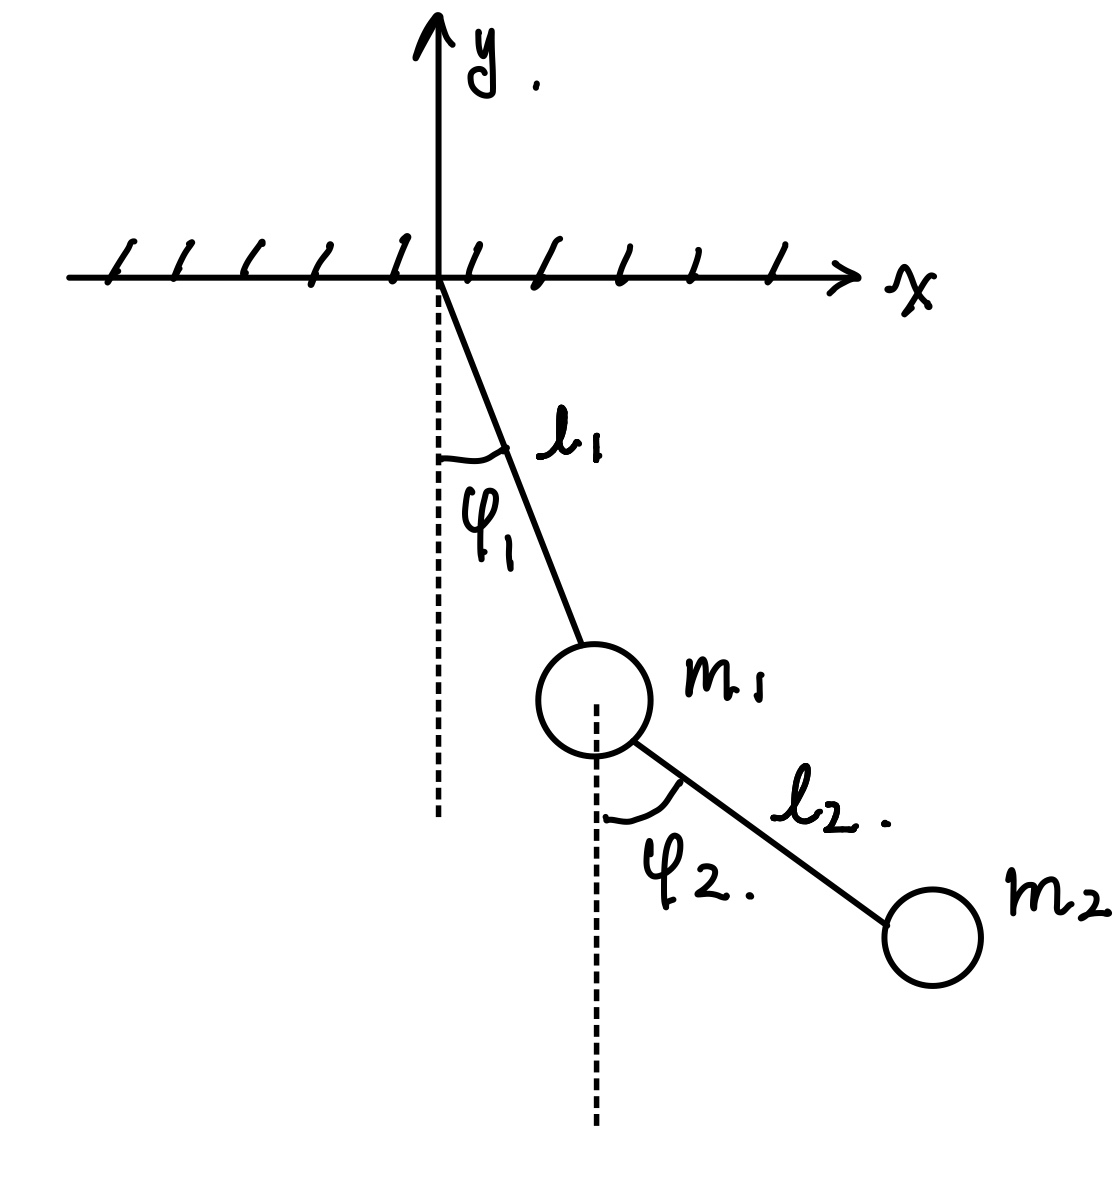
\includegraphics[scale=0.2]{Figure1.PNG}
    \caption{The double pendulum system. Assume the length of the first pendulum limb is \(\ell_1\), the length of the second pendulum limb
    is \(\ell_2\), the mass of the first bob is \(m_1\) and the mass of the second bob is \(m_2\).}
    \label{Figure 1}
\end{figure}
\begin{figure}[ht]
    \centering
    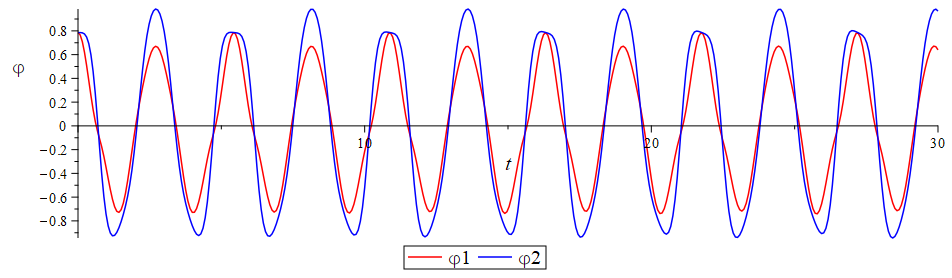
\includegraphics[scale=0.45]{Figure2.PNG}
    \caption{The angle-time plot for the solution of the non-linear equations (17) and (18) with parameters \(A = 1\), \(B= 0.5\), \(C = 9.81 \mathrm{s}^{-2}\) and initial conditions \(\varphi_1(0) = \varphi_2(0) = \pi/4\), \(\dot{\varphi}_1(0) = \dot{\varphi}_2(0) = 0\).}
    \label{Figure 2}
\end{figure}
\begin{figure}[H]
    \centering
    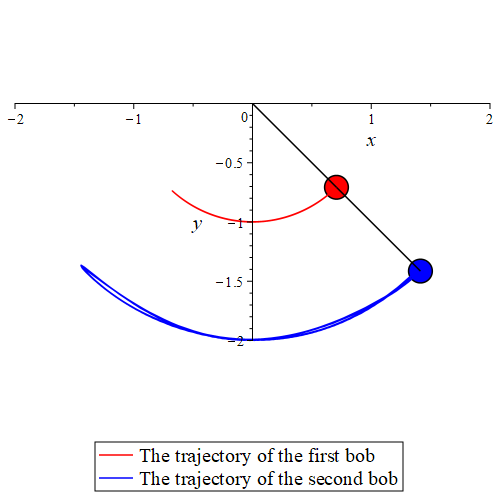
\includegraphics[scale=0.5]{Figure3.PNG}
    \caption{The trajectories of the pendulum bobs over the time interval \(0\le t\le 30\) for the solution of the non-linear equations (17) and (18) with parameters \(A = 1\), \(B= 0.5\), \(C = 9.81 \mathrm{s}^{-2}\) and initial conditions \(\varphi_1(0) = \varphi_2(0) = \pi/4\), \(\dot{\varphi}_1(0) = \dot{\varphi}_2(0) = 0\).}
    \label{Figure 3}
\end{figure}
\begin{figure}[ht]
    \centering
    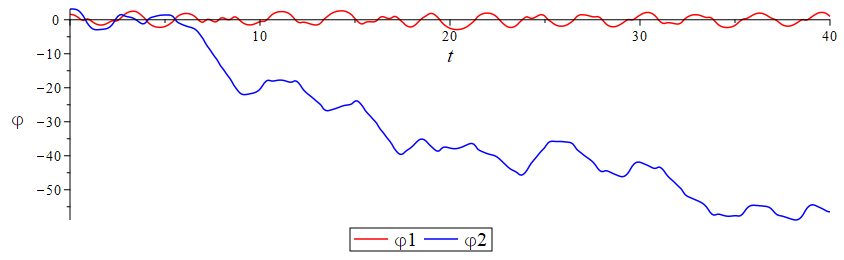
\includegraphics[scale=0.5]{Figure4.PNG}
    \caption{The angle-time plot for the solution of the non-linear equations (17) and (18) with parameters \(A = 1\), \(B= 0.5\), \(C = 9.81 \mathrm{s}^{-2}\) and initial conditions \(\varphi_1(0) = \pi/2\), \(\varphi_2(0)= \pi\), \(\dot{\varphi}_1(0) = \dot{\varphi}_2(0) = 0\).}
    \label{Figure 4}
\end{figure}
\begin{figure}[H]
    \centering
    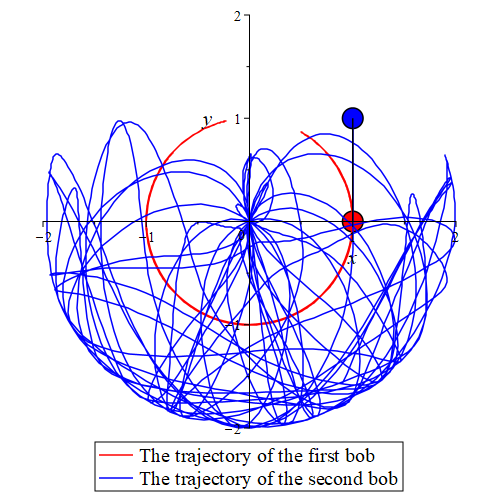
\includegraphics[scale=0.45]{Figure5.PNG}
    \caption{The trajectories of the pendulum bobs over the time interval \(0\le t\le 40\) for the solution of the non-linear equations (17) and (18) with parameters \(A = 1\), \(B= 0.5\), \(C = 9.81 \mathrm{s}^{-2}\) and initial conditions \(\varphi_1(0)=\pi/2\), \(\varphi_2(0) = \pi\), \(\dot{\varphi}_1(0) = \dot{\varphi}_2(0) = 0\).}
    \label{Figure 5}
\end{figure}
\begin{figure}[H]
    \centering
    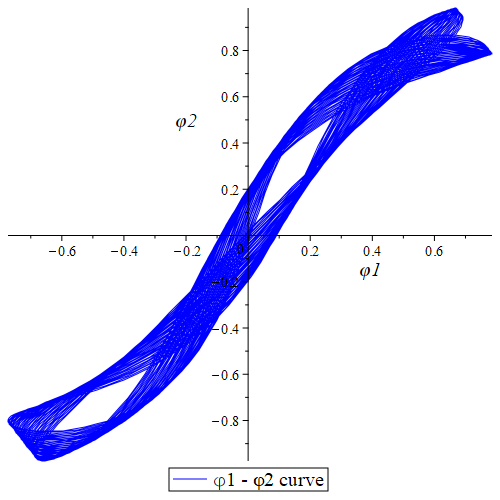
\includegraphics[scale=0.4]{Figure6.PNG}
    \caption{The \(\varphi_1 - \varphi_2\) curve over the time interval \(0\le t\le 100\) for the solution of the non-linear equations (17) and (18) with parameters \(A = 1\), \(B= 0.5\), \(C = 9.81 \mathrm{s}^{-2}\) and initial conditions \(\varphi_1(0) = \varphi_2(0) = \pi/4\), \(\dot{\varphi}_1(0) = \dot{\varphi}_2(0) = 0\).}
    \label{Figure 6}
\end{figure}
\begin{figure}[H]
    \centering
    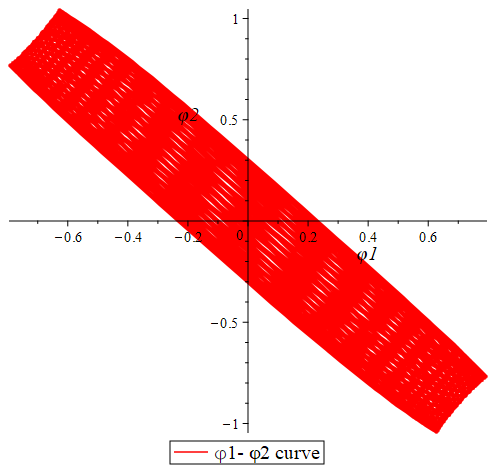
\includegraphics[scale=0.4]{Figure7.PNG}
    \caption{The \(\varphi_1 - \varphi_2\) curve over the time interval \(0\le t\le 200\) for the solution of the non-linear equations (17) and (18) with parameters \(A = 1\), \(B= 0.5\), \(C = 9.81 \mathrm{s}^{-2}\) and initial conditions \(\varphi_1(0)= -\pi/5, \varphi_2(0) = \pi/3\), \(\dot{\varphi}_1(0) = \dot{\varphi}_2(0) = 0\).}
    \label{Figure 7}
\end{figure}
\begin{figure}[ht]
    \centering
    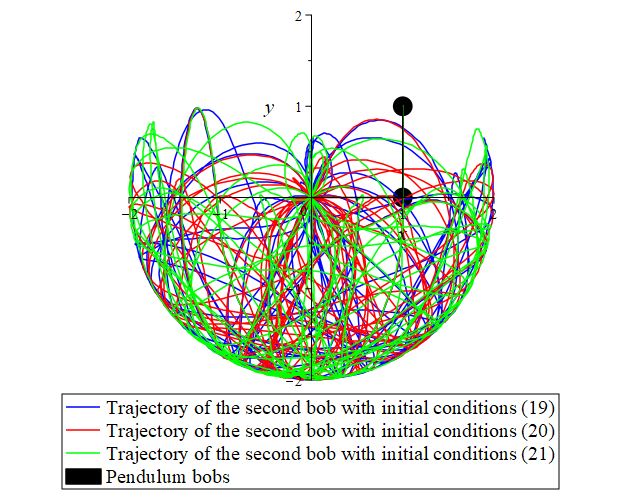
\includegraphics[scale=0.5]{Figure8.PNG}
    \caption{The trajectories of the pendulum bobs over the time interval \(0\le t\le 40\) for the solutions of the non-linear equations (17) and (18) with parameters \(A = 1\), \(B= 0.5\), \(C = 9.81 \mathrm{s}^{-2}\) and initial conditions (19), (20) and (21).}
    \label{Figure 8}
\end{figure}
\begin{figure}[H]
    \centering
    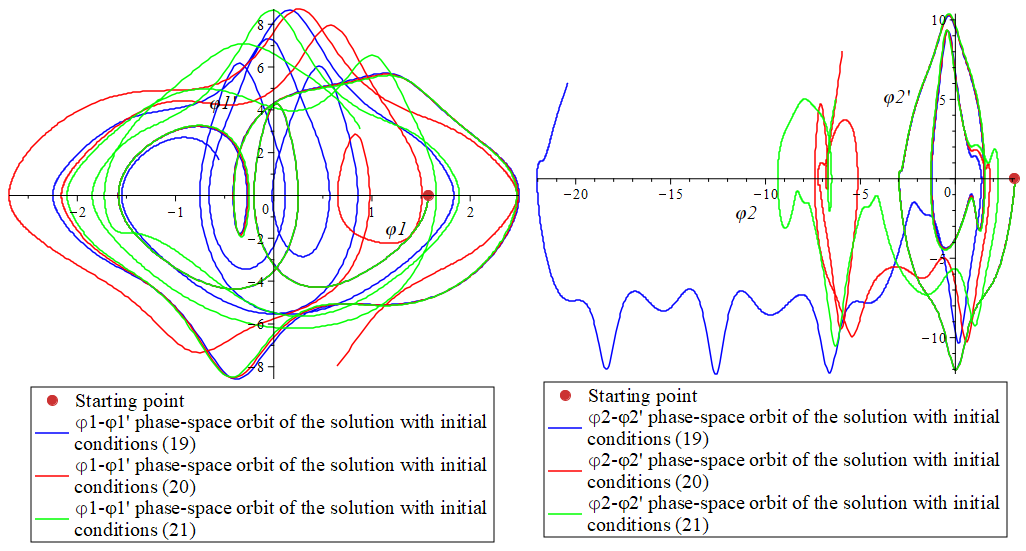
\includegraphics[scale=0.4]{Figure9.PNG}
    \caption{The phase-space orbits over the time interval \(0\le t\le 10\) for the solutions of the non-linear equations (17) and (18) with parameters \(A = 1\), \(B= 0.5\), \(C = 9.81 \mathrm{s}^{-2}\) and initial conditions (19), (20) and (21).}
    \label{Figure 9}
\end{figure}
\begin{figure}[H]
    \centering
    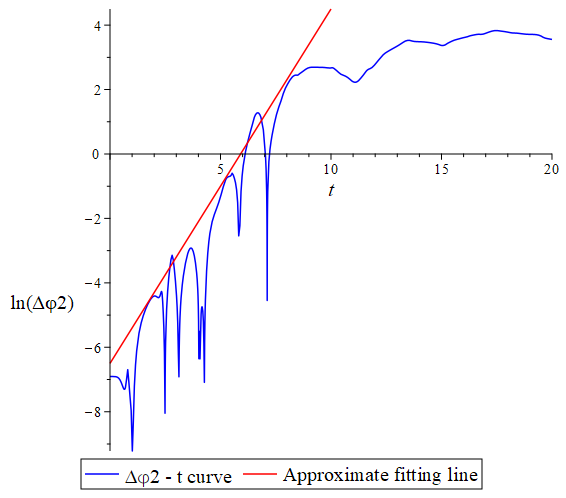
\includegraphics[scale=0.45]{Figure10.PNG}
    \caption{The \(\ln(\Delta\varphi_2(t))- t \) plot for the solutions of the non-linear equations (17) and (18) with parameters \(A = 1\), \(B= 0.5\), \(C = 9.81 \mathrm{s}^{-2}\) and initial conditions (19) and (20).}
    \label{Figure 10}
\end{figure}
\begin{thebibliography}{1}

\bibitem{Landau} Landau, L. D., Lifshitz E. M., J. B. Sykes, and J. S. Bell. \textit{Mechanics}. Pergamon Press, 1976.

\bibitem{Levin} R. B. Levien, Department of Physics, Princeton University, Princeton, New Jersey 08544 S. M. Tan, Department of
Physics, University of Auckland, Auckland, New Zealand, ``Double pendulum: An experiment in chaos", American Journal of Physics 61,
1038-1044 (1993) \url{https://doi.org/10.1119/1.17335}

\bibitem{anime} \textit{Double pendulum animation}. Stack Overflow. November 18, 2021,
\url{ https://stackoverflow.com/questions/54409094/double-pendulum-animation}.

\bibitem{Taylor} Taylor, J. R. \textit{Classical Mechanics}. University Science Books, 2005.

\bibitem{Wiki} ``Double pendulum" Wikipedia, Wikimedia Foundation, 24 September 2021,
\url{https://en.wikipedia.org/wiki/Double_pendulum#Chaotic_motion}


\end{thebibliography}
\end{document}
